% Copyright 2004 by Till Tantau <tantau@users.sourceforge.net>.
%
% In principle, this file can be redistributed and/or modified under
% the terms of the GNU Public License, version 2.
%
% However, this file is supposed to be a template to be modified
% for your own needs. For this reason, if you use this file as a
% template and not specifically distribute it as part of a another
% package/program, I grant the extra permission to freely copy and
% modify this file as you see fit and even to delete this copyright
% notice. 

\documentclass{beamer}
\usepackage{boondox-cal}
\usepackage{tikz}
\usetikzlibrary{bayesnet}
\usepackage{kotex}
\usepackage{amsfonts}
\usepackage{subcaption}
\captionsetup{compatibility=false}
\usepackage{amssymb}
\newcommand{\E}{\mathbb{E}}
\usepackage{amsthm}
\usepackage{latexsym,amsmath}
\usepackage{graphicx}
\usepackage{pgfplots}
\usepackage{afterpage}
\usepackage[ ]{algorithm2e}
\usepackage{bm}
\newcommand{\R}{\mathbb{R}}
\DeclareMathOperator*{\argmin}{arg\,min}
% There are many different themes available for Beamer. A comprehensive
% list with examples is given here:
% http://deic.uab.es/~iblanes/beamer_gallery/index_by_theme.html
% You can uncomment the themes below if you would like to use a different
% one:
%\usetheme{AnnArbor}
%\usetheme{Antibes}
%\usetheme{Bergen}
%\usetheme{Berkeley}
%\usetheme{Berlin}
%\usetheme{Boadilla}
%\usetheme{boxes}
%\usetheme{CambridgeUS}
%\usetheme{Copenhagen}
%\usetheme{Darmstadt}
%\usetheme{default}
%\usetheme{Frankfurt}
%\usetheme{Goettingen}
%\usetheme{Hannover}
%\usetheme{Ilmenau}
%\usetheme{JuanLesPins}
%\usetheme{Luebeck}
\usetheme{Madrid}
%\usetheme{Malmoe}
%\usetheme{Marburg}
%\usetheme{Montpellier}
%\usetheme{PaloAlto}
%\usetheme{Pittsburgh}
%\usetheme{Rochester}
%\usetheme{Singapore}
%\usetheme{Szeged}
%\usetheme{Warsaw}

\title{Density Ratio Estimators in Variational Bayesian Machine Learning}

% A subtitle is optional and this may be deleted
%\subtitle{Optional Subtitle}

\author{Lammy}
% - Give the names in the same order as the appear in the paper.
% - Use the \inst{?} command only if the authors have different
%   affiliation.

\institute[UNSW] % (optional, but mostly needed)
{
  Department of Mathematics and Statistics\\
  UNSW
  }
% - Use the \inst command only if there are several affiliations.
% - Keep it simple, no one is interested in your street address.

\date{Statistics Honours, 2018}
% - Either use conference name or its abbreviation.
% - Not really informative to the audience, more for people (including
%   yourself) who are reading the slides online

\subject{Statistics}
% This is only inserted into the PDF information catalog. Can be left
% out. 

% If you have a file called "university-logo-filename.xxx", where xxx
% is a graphic format that can be processed by latex or pdflatex,
% resp., then you can add a logo as follows:

% \pgfdeclareimage[height=0.5cm]{university-logo}{university-logo-filename}
% \logo{\pgfuseimage{university-logo}}

% Delete this, if you do not want the table of contents to pop up at
% the beginning of each subsection:
\AtBeginSubsection[]
{
  \begin{frame}<beamer>{Outline}
    \tableofcontents[currentsection,currentsubsection]
  \end{frame}
}

% Let's get started
\begin{document}

\begin{frame}
  \titlepage
\end{frame}

\begin{frame}{Outline}
  \tableofcontents
  % You might wish to add the option [pausesections]
\end{frame}

% Section and subsections will appear in the presentation overview
% and table of contents.
\section{Background Info}

\subsection{Neural Networks}

\begin{frame}{Neural Networks}{Overall Structure}
  \begin{itemize}
  \item {
    Mathematical model based off human brain.
  }
  \item {
  	Letting $f^*$ be some function in $\R$, goal of neural network is to approximate $f^*$ using a mapping with parameters $\bm{\Theta}$ from input $\bm{x}$ to output $\bm{y}$: $\bm{y}=\bm{f}_{\bm{\Theta}}(\bm{x})$.
  }
  \item {
  	Universal Approximation Theorem states a neural network can approximate any function if it is complex enough.
  }
  \item {
    Consists of layers of nodes:
  }
  \begin{figure}[h]
  \resizebox{.5\linewidth}{!}{
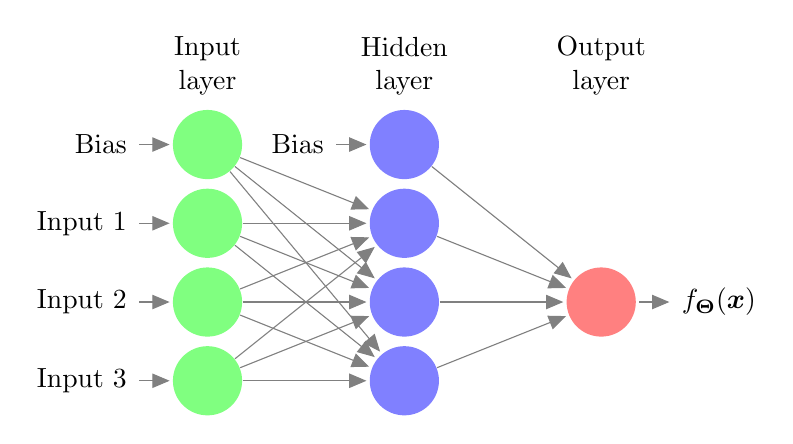
\begin{tikzpicture}[shorten >=1pt,->,draw=black!50, node distance=2.5cm]
    \tikzstyle{every pin edge}=[<-,shorten <=1pt]
    \tikzstyle{neuron}=[circle,fill=black!25,minimum size=25pt,inner sep=0pt]
    \tikzstyle{input neuron}=[neuron, fill=green!50];
    \tikzstyle{output neuron}=[neuron, fill=red!50];
    \tikzstyle{hidden neuron}=[neuron, fill=blue!50];
    \tikzstyle{annot} = [text width=4em, text centered]
    
	\node[input neuron, pin=left:Bias] (I-0) at (0,0) {};
    % Draw the input layer nodes
    \foreach \name / \y in {1,...,3}
    % This is the same as writing \foreach \name / \y in {1/1,2/2,3/3,4/4}
        \node[input neuron, pin=left:Input \y] (I-\name) at (0,-\y) {};

 \path[yshift=0cm]
            node[hidden neuron, pin=left:Bias] (H-0) at (2.5cm,0) {};
    % Draw the hidden layer nodes
    \foreach \name / \y in {1,...,3}
        \path[yshift=0cm]
            node[hidden neuron] (H-\name) at (2.5cm,-\y) {};

    % Draw the output layer node
	\path[yshift=1cm]    
    node[output neuron,pin={[pin edge={->}]right:$f_{\bm{\Theta}}(\bm{x})$}, right of=H-2] (O) {};

    % Connect every node in the input layer with every node in the
    % hidden layer.
    \foreach \source in {0,...,3}
        \foreach \dest in {1,...,3}
            \path (I-\source) edge (H-\dest);

    % Connect every node in the hidden layer with the output layer
    \foreach \source in {0,...,3}
        \path (H-\source) edge (O);

    % Annotate the layers
    \node[annot,above of=H-0, node distance=1cm] (hl) {Hidden layer};
    \node[annot,left of=hl] {Input layer};
    \node[annot,right of=hl] {Output layer};
\end{tikzpicture}
}
\end{figure}
  \end{itemize}
  
\end{frame}
\begin{frame}{Neural Networks}{Individual Node Structure}
\begin{itemize}
\item Each node is a generalised linear model of preceding layer output.
\item Weights $\theta$ are randomly initialised from normal or uniform distribution.
\item Bias $x_0=1$ has role of intercept term in typical regression.
\begin{figure}[h]
  \resizebox{.4\linewidth}{!}{
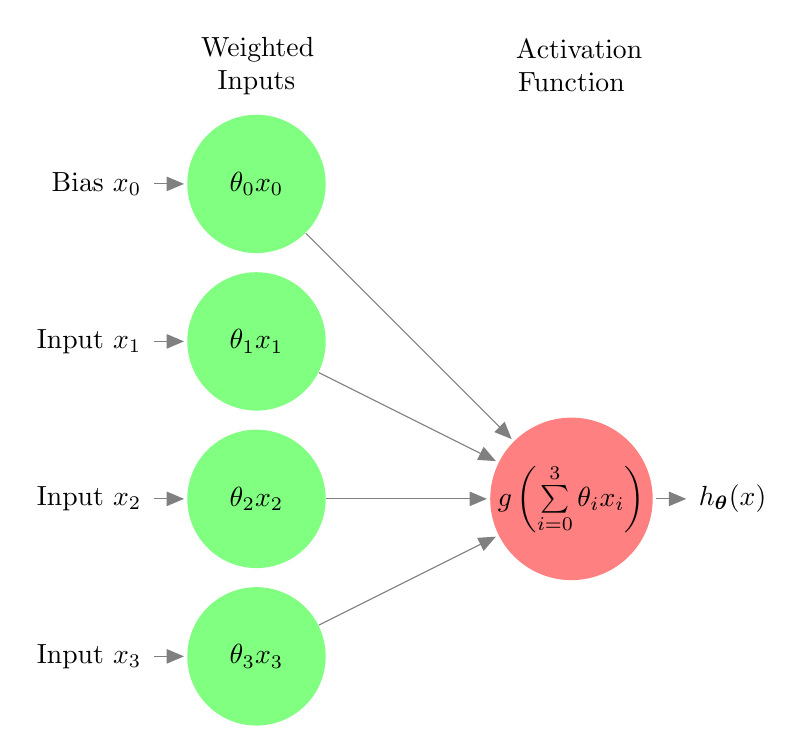
\begin{tikzpicture}[shorten >=1pt,->,draw=black!50, node distance=2.5cm]
    \tikzstyle{every pin edge}=[<-,shorten <=1pt]
    \tikzstyle{neuron}=[circle,fill=black!25,minimum size=50pt,inner sep=0pt]
    \tikzstyle{input neuron}=[neuron, fill=green!50];
    \tikzstyle{output neuron}=[neuron, fill=red!50];
    \tikzstyle{hidden neuron}=[neuron, fill=blue!50];
    \tikzstyle{annot} = [text width=4em, text centered]

    % Draw the input layer nodes
 %   \foreach \name / \y in {0,...,3}
    % This is the same as writing \foreach \name / \y in {1/1,2/2,3/3,4/4}
        \node[input neuron, pin=left:Bias $x_0$] (I-0) at (0,-0) {$\theta_0 x_0$};
	\foreach \name / \y in {1,...,3}
    % This is the same as writing \foreach \name / \y in {1/1,2/2,3/3,4/4}
        \node[input neuron, pin=left:Input $x_{\y}$] (I-\name) at (0,-2*\y) {$\theta_{\y}x_\y$};
    % Draw the hidden layer nodes
    %\foreach \name / \y in {1,...,5}
     %   \path[yshift=0.5cm]
      %      node[hidden neuron] (H-\name) at (\layersep,-\y cm) {};

    % Draw the output layer node
    \node[output neuron,pin={[pin edge={->}]right:$h_{\bm{\theta}}(x)$}, right of=I-2, node distance=4cm] (O) {$g\left(\sum\limits^3_{i=0}\theta_ix_i\right)$};

    % Connect every node in the input layer with every node in the
    % hidden layer.
   % \foreach \source in {1,...,4}
    %    \foreach \dest in {1,...,5}
     %       \path (I-\source) edge (H-\dest);

    % Connect every node in the hidden layer with the output layer
    \foreach \source in {0,...,3}
        \path (I-\source) edge (O);

    % Annotate the layers
%    \node[annot,above of=H-1, node distance=1cm] (hl) {Hidden layer};
    \node[annot,above of=I-0, node distance=1.5cm](il) {Weighted Inputs};
    \node[annot,right of=il, node distance=4cm] {Activation Function};
\end{tikzpicture}
}
\end{figure}

\end{itemize}
\end{frame}
\begin{frame}{Neural Networks}{Activation Functions}
\begin{itemize}
\item Used to map node output to certain space.
\item Every node except input nodes has an activation function.
\item We are mostly concerned with activation function of output layer, which maps $\R$ to some space:
\begin{itemize}
\item Linear (no) activation function $g(x)=x$ outputs in $\R$.
\item Rectified Linear Unit (ReLU) activation function $g(x)=\max\{0,x\}$ in $[0,\infty)$.
\item Sigmoid activation function $g(x)=(1+\exp(-x))^{-1}$ in $(0,1)$.
\end{itemize}
\end{itemize}
\end{frame}
\begin{frame}{Neural Networks}{Training}
\begin{itemize}
\item Weights and biases trained such that (ideally convex) loss function is minimized e.g. Mean Squared Error: $\min_\Theta \frac{1}{2}||\bm{y}-\bm{f}_\Theta(\bm{x})||^2_2$.
\item Back-propagation finds partial derivatives of loss function with respect to weights by propagating error backwards through network.
\item Gradient descent uses these partial derivatives to optimize network.
\end{itemize}
\end{frame}
\subsection{(Amortized) Variational Inference}

% You can reveal the parts of a slide one at a time
% with the \pause command:
\begin{frame}{(Amortized) Variational Inference}{Bayesian Inference}
  \begin{itemize}
  \item {
    Fundamental problem in Bayesian computation is to estimate posterior densities $p(z|x)$.
    %\pause % The slide will pause after showing the first item
  }
  \begin{equation*}
p(z|x)=\frac{p(z,x)}{p(x)}= \frac{p(z)p(x|z)}{\int_\mathcal{z}p(z,x)dz}
\end{equation*}
  \item {   
    Problems arise when $\int_\mathcal{z}p(z,x)dz$ is computationally intractable.
  }
  % You can also specify when the content should appear
  % by using <n->:
  \item {
    Typical MCMC methods are slow with large datasets or high dimensional data.
  }
  % or you can use the \uncover command to reveal general
  % content (not just \items):
  \item {
    Variational Inference is a solution.
  }
  \end{itemize}
\end{frame}
\begin{frame}{(Amortized) Variational Inference}{Introduction}
\begin{itemize}
\item Amortized variational inference approximates $p(z|x)$ with a different distribution $q_\phi(z|x)$.
\item $q_\phi(z|x)$ is a neural network with parameters $\phi$ that takes in data $x$ and random noise $\epsilon\sim \pi(\epsilon)$ and outputs samples $z\sim q_\phi(z|x)$.
\item Typically $\pi(\epsilon)=\mathcal{N}(0,I_{n\times n})$.
\begin{figure}[h]
  \centering
  \tikz{ %
    \node[latent] (x) {$x$} ; %
    \node[det, right=of x] (q) {$q_\phi(z|x)$} ; %
    \node[latent, right=of q] (qout) {$z$} ;
    \node [latent, above=of x] (eps) {$\epsilon$} ;
    \edge {x} {q} ; %
    \edge {eps} {q} ;
    \edge {q} {qout} ;
  }
\end{figure}
\end{itemize}
\end{frame}
\begin{frame}{(Amortized) Variational Inference}{Network Training}
\begin{itemize}
\item Minimize (reverse) KL Divergence between the two distributions. Since $p(z|x)$ changes with different $x$, take expectation with respect to dataset $q^*(x)$:
\begin{equation*}
q^*_\phi(z|x)=\argmin_{q(z|x)\in \mathcal{Q}}\E_{q^*(x)}[KL(q_\phi(z|x)||p(z|x))].
\end{equation*}
\item Reverse KL Divergence is the expected logarithmic difference between two distributions P and Q with respect to Q:
\[KL(q(z|x)||p(z|x))=\mathbb{E}_{q(z|x)}\left[\log \left(\frac{q(z|x)}{p(z|x)}\right)\right]\].
\end{itemize}
\end{frame}
\begin{frame}{(Amortized) Variational Inference}{Network Training}
\begin{itemize}
\item We don't know $p(z|x)$ so we apply Bayes' law to $p(z|x)$ and move out intractable $\log p(x)$ term.
\small
\begin{align*}
\E_{q^*(x)}[KL(q_\phi(z|x)||&p(z|x))]\\
&=\mathbb{E}_{q^*(x)q_\phi(z|x)}[\log q(z)-\log p(x|z)-\log p(z)+\log p(x)]
\end{align*}
\begin{align*}
\E_{q^*(x)}[KL(q_\phi(z|x)||&p(z|x))-\log p(x)]\\
&=-\mathbb{E}_{q^*(x)q(z)}[\log p(x|z)]+\E_{q^*(x)}KL[q_\phi(z|x)||p(z)]
\end{align*}
\normalsize
\item Denote RHS as $NELBO(q)$, the \textbf{n}egative of the \textbf{e}vidence \textbf{l}ower \textbf{bo}und:
\[\min_\phi NELBO(q)=-\mathbb{E}_{q_\phi(z|x)q^*(x)}[\log p(x|z)]+\mathbb{E}_{q^*(x)}[KL(q_\phi(z|x)||p(z))].\]
\end{itemize}
\end{frame}
\begin{frame}{(Amortized) Variational Inference}{Prior-Contrastive}
\[\min_\phi -\mathbb{E}_{q_\phi(z|x)q^*(x)}[\log p(x|z)]+\mathbb{E}_{q^*(x)}[KL(q_\phi(z|x)||p(z))].\]
\begin{itemize}
\item $q_\phi(z|x)$ is a neural network so extremely difficult to find explicit form, we therefore say that it is \textbf{implicit}.
\item Use density ratio estimation to evaluate $\frac{q_\phi(z|x)}{p(z)}$ in $KL(q_\phi(z|x)||p(z))$.
\item The prior $p(z)$ can therefore be implicit.
\item We call this the ``prior-contrastive" formulation.
\end{itemize}
\end{frame}
\begin{frame}{(Amortized) Variational Inference}{Joint-Contrastive}
\begin{itemize}
\item If the likelihood $p(x|z)$ is implicit, then our optimization problem is \[\min_\phi KL(q(z,x)||p(z,x)).\]
\item Use density ratio estimation to evaluate $\frac{q(z,x)}{p(z,x)}$.
\item For consistency, $NELBO(q)=\min_\phi KL(q(z,x)||p(z,x))$.
\item We call this the ``joint-contrastive" formulation.
\end{itemize}
\end{frame}
%\begin{frame}{(Amortized) Variational Inference}{Autoencoders}
%\begin{itemize}
%\item An autoencoder consists of an encoder $q_\phi(z|x)$ that `compresses' data $x$ into lower dimensional latent $z$, and a decoder $p_\theta(x|z)$ that generates data $x$ from $z$.
%\item This is the same as our Bayesian inference problem except the likelihood is a neural network parametrised with $\theta$.
%\item To generate new data, sample $z\sim p(z)$ and pass through decoder.
%\item We typically know $p_\theta(x|z)$ in explicit form e.g. if $x$ is grey-scale image data, then $p_\theta(x|z)$ is a Bernoulli distribution with parameters given by sigmoid output of the neural network.
%\item Therefore have optimization problem $\min_{\theta, \phi} -\mathbb{E}_{q_\phi(z|x)q^*(x)}[\log p_\theta(x|z)]+\mathbb{E}_{q^*(x)}[KL(q_\phi(z|x)||p(z))].$
%\item If $p_\theta(x|z)$ is implicit then we have the optimization problems $\min_\phi KL(q(z,x)||p(z,x))$ and $\min_\theta KL(p(z,x)||q(z,x))$.
%\end{itemize}
%\end{frame}
\subsection{Density Ratio Estimation}

% You can reveal the parts of a slide one at a time
% with the \pause command:
\begin{frame}{Density Ratio Estimation}{Class Probability Estimation}
We want to estimate $\frac{q(u)}{p(u)}$.
  \begin{enumerate}
  \item {
    Define discriminator function that finds probability that a sample $u$ came from $q(u)$: $D_\alpha(u)\simeq P(u\sim q(u))$, so that $\frac{q(u)}{p(u)}\simeq \frac{D_\alpha(u)}{1-D_\alpha(u)}$.
  }
  \item $D_\alpha(u)$ is neural network parametrised by $\alpha$, sigmoid activation function used for output layer
  % or you can use the \uncover command to reveal general
  % content (not just \items):
  \item {
    Train discriminator with Bernoulli loss: $\min_\alpha -\mathbb{E}_{q(u)}[\log D_\alpha(u)]-\mathbb{E}_{p(u)}[\log(1-D_\alpha(u))]$.
  }
  \item Optimal discriminator is $D^*_\alpha(u)=\frac{q(u)}{q(u)+p(u)}$.
  \end{enumerate}
\end{frame}
\begin{frame}{Density Ratio Estimation}{Class Probability Estimation}
Prior-Contrastive Application:
\[\min_\alpha -\mathbb{E}_{q^*(x)q_\phi(z|x)}[\log D_\alpha(z,x)]-\mathbb{E}_{q^*(x)p_\theta(z)}[\log (1-D_\alpha(z,x))]\]
\[\min_\phi -\mathbb{E}_{q^*(x)q_\phi(z|x)}[\log p(x|z)]+\mathbb{E}_{q^*(x)q_\phi(z|x)}\left[\log \frac{D_\alpha(z,x)}{1-D_\alpha(z,x)}\right]\]
Joint-Contrastive Application:
\[\min_\alpha -\mathbb{E}_{q^*(x)q_\phi(z|x)}[\log D_\alpha(z,x)]-\mathbb{E}_{p(z)p(x|z)}[\log (1-D_\alpha(z,x))]\]
\[\min_\phi \mathbb{E}_{q^*(x)q_\phi(z|x)}\log\frac{D_\alpha(z,x)}{1-D_\alpha(z,x)}\]
Program alternates between several optimisation steps of discriminator and one optimisation step of posterior.
\end{frame}
\begin{frame}{Density Ratio Estimation}{Divergence Minimisation}
\begin{theorem}
If $f$ is a convex function with derivative $f'$ and convex conjugate $f^*$, and $\mathcal{R}$ is a class of functions with codomains equal to the domain of $f'$, then we have the lower bound for the f-divergence between distributions $p(u)$ and $q(u)$:
\[D_f [p(u)||q(u)]\geq \sup_{r\in \mathcal{R}} \{\mathbb{E}_{q(u)}[f'(r(u))]-\mathbb{E}_{p(u)}[f^*(f'(r(u)))]\},\]
with equality when $r(u)=q(u)/p(u)$.
\end{theorem}
For the reverse KL divergence, $f(u)=u\log u$ so we have
\[KL[q(u)||p(u)]\geq \sup_{r\in \mathcal{R}}\{\mathbb{E}_{q(u)}[1+\log r(u)]-\mathbb{E}_{p(u)}[r(u)]\}\]

\end{frame}
\begin{frame}{Density Ratio Estimation}{Divergence Minimisation}
\begin{itemize}
\item Let our ratio estimator be a neural network parametrised by $\alpha$: $r_\alpha(u)\simeq \frac{q(u)}{p(u)}$.
\item Maximise the lower bound w.r.t. $\alpha$ until equality, which is when $r_\alpha(u)=\frac{q(u)}{p(u)}$. The optimisation problem for this is
\[\min_\alpha -\mathbb{E}_{q(u)}[\log r_\alpha(u)]+\mathbb{E}_{p(u)}[r_\alpha(u)].\]
\item Obviously our optimal ratio estimator is $r^*_\alpha(u)=\frac{q(u)}{p(u)}$.
\end{itemize}
\end{frame}
\begin{frame}{Density Ratio Estimation}{Divergence Minimisation}
Prior-Contrastive Application:
\[\min_\alpha -\E_{q^*(x)q_\phi(z|x)}[\log r_\alpha(z,x)]+\E_{q^*(x)p(z)}[r_\alpha (z,x)]\]
\[\min_\phi -\mathbb{E}_{q^*(x)q_\phi(z|x)}\left[\log p(x|z)\right]+E_{q^*(x)q_\phi (z|x)}[\log r_\alpha(z,x)]\]
Joint-Contrastive Application:
\[\min_\alpha-\E_{q^*(x)q_\phi(z|x)}[\log r_\alpha(z,x)]+\E_{p(z)p(x|z)}[r_\alpha(z,x)]\]
\[\min_\phi \mathbb{E}_{q^*(x)q_\phi(z|x)}[\log r_\alpha(z,x)]\]
\end{frame}
\section{Activation Function Experiment}
\begin{frame}{Activation Function Experiment}{Experiment Outline}
\[p(z_1,z_2)\sim \mathcal{N} (0,\sigma^2 I_{2\times 2})\]
\[p(x|\bm{z})\sim EXP(3+\max(0,z_1)^3+\max(0,z_2)^3)\]
\begin{figure}[h]
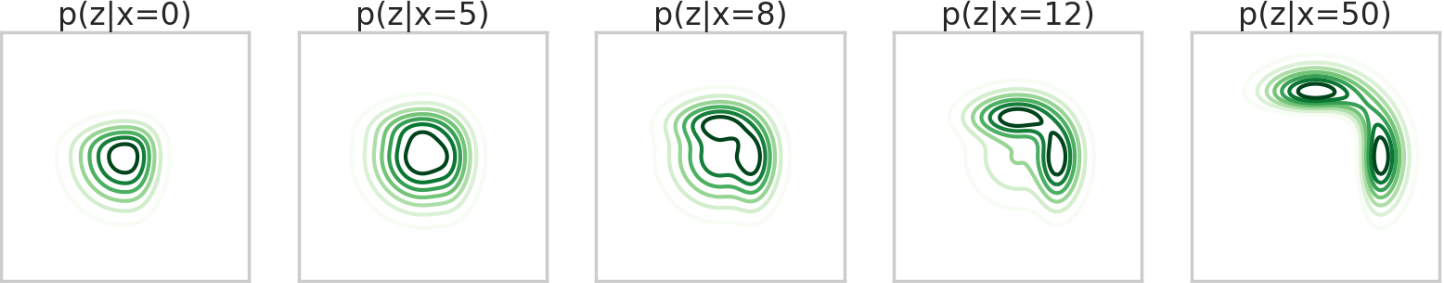
\includegraphics[width=\textwidth]{sprinklertrue.png}
\end{figure}
\begin{itemize}
\item Posterior is flexible and bimodal.
\item Use Gaussian KDE to find `true' KL divergence for $q_\phi(z|x=0,5,8,12,50)$.
\end{itemize}
\end{frame}
%\begin{frame}{Inference Experiment}{Experiment Outline}
%Class Probability Estimation vs Divergence Minimisation
%\begin{itemize}
%\item Learning rate of 0.0001 for prior-contrastive and 0.00001 for joint-contrastive.
%\item 5000 training steps of estimator for initialisation, then alternation between 100 estimator steps and 1 posterior step for 10000 posterior iterations in prior-contrastive and 40000 posterior iterations in joint-contrastive.
%\item Sigmoid output activation function for class probability estimation and ReLU output for divergence minimisation.
%\item Only trained on data values $x=0,5,8,12,50$, with 200 samples of each taken per training batch (training batch size is 1000).
%\item Both algorithms have identical neural network structure and runtime.
%\item Small constant of $c=10^{-18}$ added to log function input to prevent $\log 0$.
%\end{itemize}
%\end{frame}
%\begin{frame}{Initial Inference Experiment}{Results}
%\begin{itemize}
%\item Estimator loss and estimated NELBO recorded every iteration.
%\item Gaussian kernel density estimator $\hat{q}_\phi(z|x)$ used to estimate posterior density for $x=0,5,8,12,50$, and average KL divergence between these 5 values was recorded every 100 iterations.
%\item Experiment repeated 30 times and the 3 arrays of recorded values were averaged.
%\end{itemize}
%\begin{table}[h]
%\scalebox{0.8}{
%\begin{tabular}{|c|c|c|}
%\hline
%Algorithm & Mean KL Divergence & Standard Deviation\\
%\hline
%PC Divergence Minimisation & 1.3807 & 0.0391\\
%\hline
%PC Class Probability Estimation & 1.3267 & 0.0041\\
%\hline
%JC Divergence Minimisation & 1.6954 & 0.4337\\
%\hline
%JC Class Probability Estimation & 1.3925 & 0.0669\\
%\hline
%\end{tabular}
%}
%\end{table}
%
%\end{frame}
%\begin{frame}{Initial Inference Experiment}{Example Posterior Outputs}
%
%\begin{figure}[h]
%\scalebox{0.8}{
%\begin{subfigure}{\textwidth}
%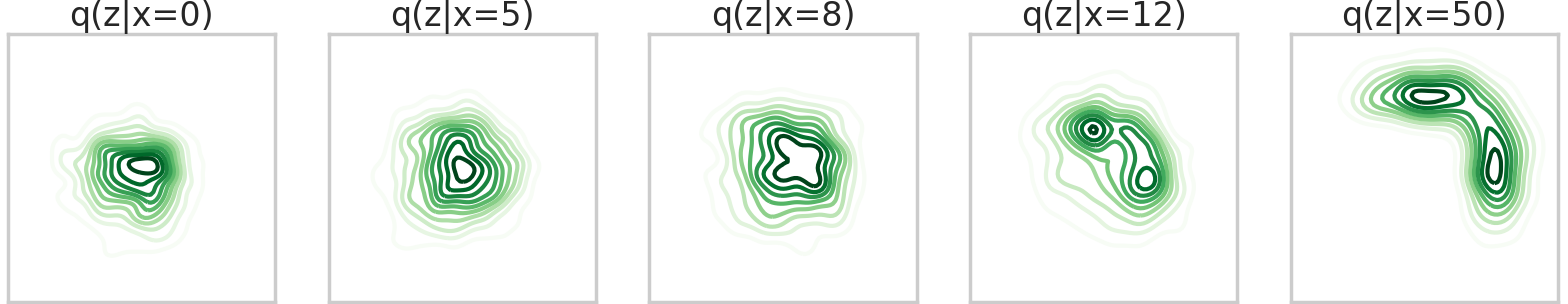
\includegraphics[width=\textwidth]{13288.png}
%\caption{Average KL Divergence of 1.3288}
%\end{subfigure}
%}
%\scalebox{0.8}{
%\begin{subfigure}{\textwidth}
%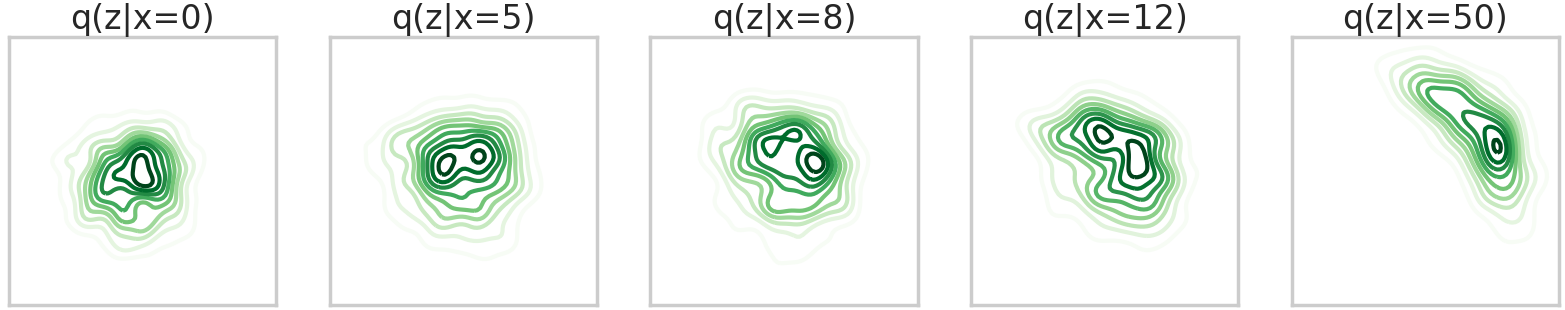
\includegraphics[width=\textwidth]{13963.png}
%\caption{Average KL Divergence of 1.3963}
%\end{subfigure}
%}
%\scalebox{0.8}{
%\begin{subfigure}{\textwidth}
%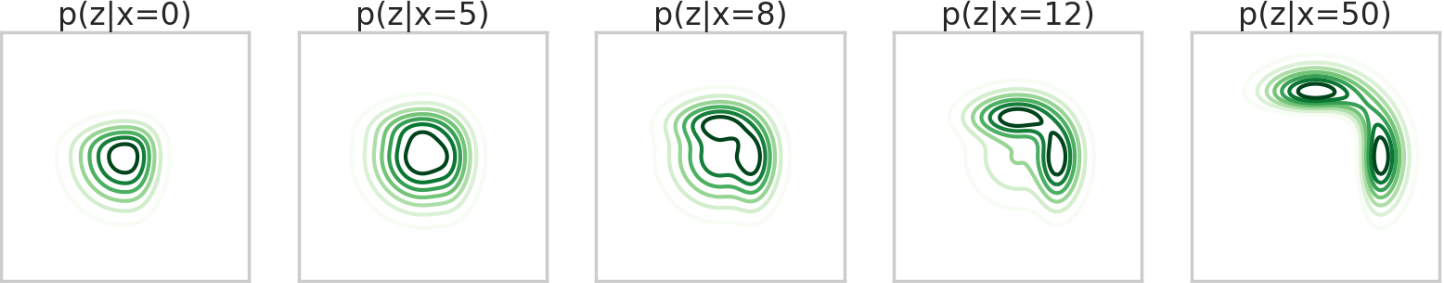
\includegraphics[width=\textwidth]{sprinklertrue}
%\caption{True Posterior Plot}
%\end{subfigure}
%}
%\end{figure}
%\end{frame}
%\begin{frame}{Initial Inference Experiment}{KL Divergence Plots}
%\begin{figure}
%\begin{subfigure}{0.49\textwidth}
%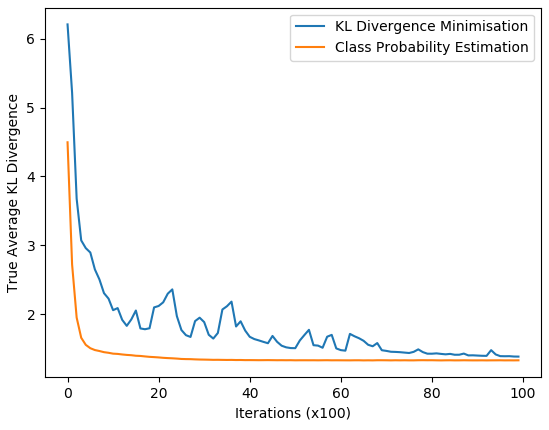
\includegraphics[width=\linewidth]{truklmins/PCKLvsPCADV.png}
%\caption{Prior-Contrastive}
%\end{subfigure}
%\begin{subfigure}{0.49\textwidth}
%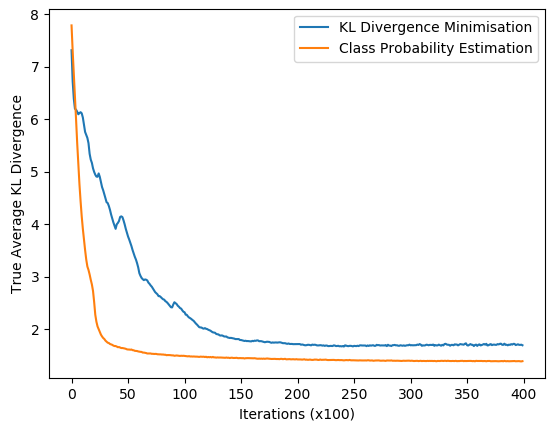
\includegraphics[width=\linewidth]{truklmins/JCKLvsJCADV.png}
%\caption{Joint-Contrastive}
%\end{subfigure}
%\end{figure}
%\end{frame}
%\begin{frame}{Initial Inference Experiment}{Estimator Losses}
%\begin{figure}
%\begin{subfigure}{0.49\textwidth}
%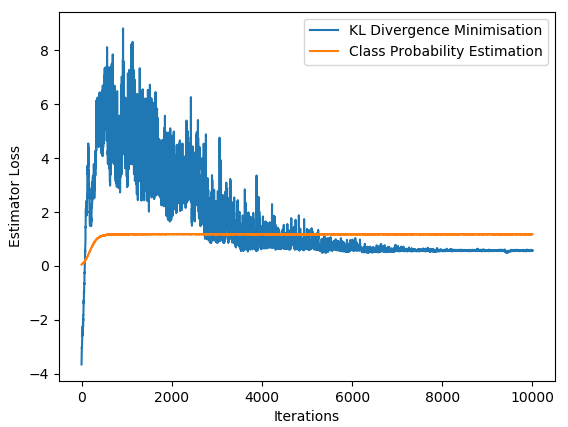
\includegraphics[width=\linewidth]{estimator_losses/PCKLvsPCADV.png}
%\caption{Prior-Contrastive}
%\end{subfigure}
%\begin{subfigure}{0.49\textwidth}
%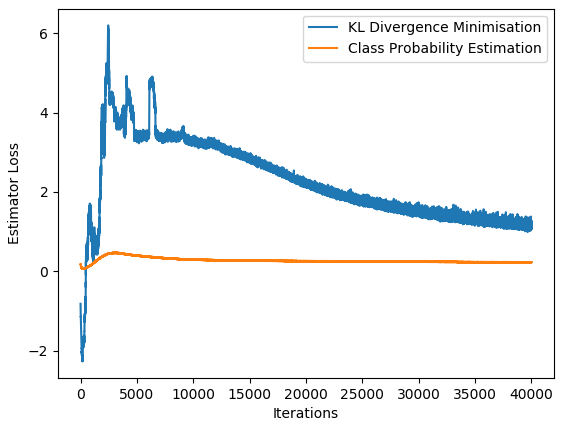
\includegraphics[width=\linewidth]{estimator_losses/JCKLvsJCADV.png}
%\caption{Joint-Contrastive}
%\end{subfigure}
%\end{figure}
%\end{frame}
%\begin{frame}{Initial Inference Experiment}{NELBOs}
%\begin{figure}
%\begin{subfigure}{0.49\textwidth}
%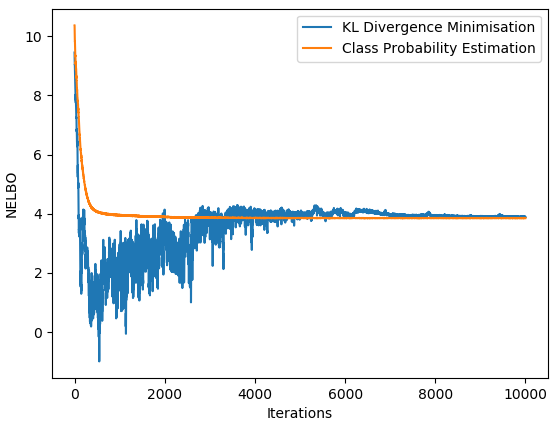
\includegraphics[width=\linewidth]{nelbos/PCKLvsPCADV.png}
%\caption{Prior-Contrastive}
%\end{subfigure}
%\begin{subfigure}{0.49\textwidth}
%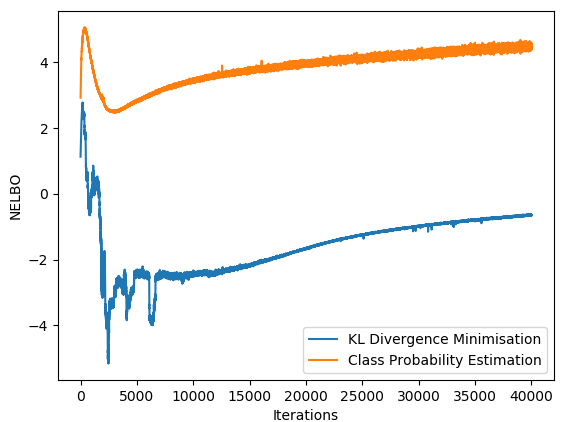
\includegraphics[width=\linewidth]{nelbos/JCKLvsJCADV.png}
%\caption{Joint-Contrastive}
%\end{subfigure}
%\end{figure}
%\end{frame}
\begin{frame}{Activation Function Experiment}{Failures}
\begin{itemize}
\item Divergence Minimisation regularly experienced `failures'
\item Estimator loss initialised at $41.4465$ and remained constant over optimisation steps.
\item Analysis of estimator output showed that it was outputting negative number which was mapped to $0$ by ReLU.
\item Recall ratio estimator loss of $-\E_q[\log r_\alpha(z,x)+\E_p[r_\alpha(z,x)]$.
\item We added constant term of $c=10^{-18}$ to log input.
\item $-\log 10^{-18}=41.4465$
\item Partial derivative of loss function w.r.t weights is $0$ as changing weight values slightly still results in negative output before ReLU.
\end{itemize}
\end{frame}
\begin{frame}{Activation Function Experiment}{Problems with ReLU}
\begin{itemize}
\item `Failures' caused from ReLU outputting in $[0,\infty)$ despite $\frac{q(u)}{p(u)}\in (0,\infty)$.
\item If $q(u)<p(u)$, $\frac{q(u)}{p(u)}\in (0,1)$, and if $q(u)>p(u)$, $\frac{q(u)}{p(u)}\in (1,\infty)$.
\item Linearity of ReLU activation results in inconsistent training, as small training steps should be taken if $q(u)<p(u)$, but large training steps required for $q(u)>p(u)$.
\end{itemize}
\end{frame}
\begin{frame}{Activation Function Experiment}{Parameters}
\begin{itemize}
\item First contribution of thesis: we propose exponential activation function $g(x)=e^x$ for ratio estimator.
\item This maps $\R^-$ to $(0,1)$, and $\R^+$ to $(1,\infty)$.
\item Training is consistent and neural network cannot output $0$.
\item Compare ReLU vs exp activation function for divergence minimisation.
\item Low training rate, high iterations to ensure smooth convergence.
\end{itemize}
\end{frame}
\begin{frame}{Activation Function Experiment}{Results}
\begin{table}[h]
\scalebox{0.8}{
\begin{tabular}{|c|c|c|}
\hline
Algorithm & Mean KL Divergence & Standard Deviation\\
\hline
PC Divergence Minimisation - ReLU & 1.3807 & 0.0391\\
\hline
PC Divergence Minimisation - Exp & 1.3265 & 0.0045\\
\hline
JC Divergence Minimisation - ReLU & 1.6954 & 0.4337\\
\hline
JC Divergence Minimisation - Exp & 1.3397 & 0.0066\\
\hline
\end{tabular}
}
\end{table}
\begin{figure}[h]
\scalebox{0.8}{
\begin{subfigure}{\textwidth}
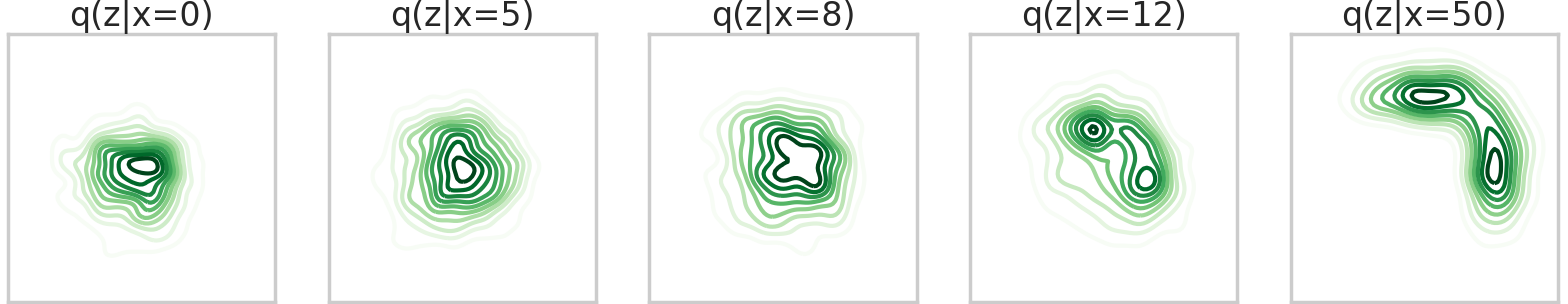
\includegraphics[width=\textwidth]{13288.png}
\caption{Average KL Divergence of 1.3288}
\end{subfigure}
}
\scalebox{0.8}{
\begin{subfigure}{\textwidth}
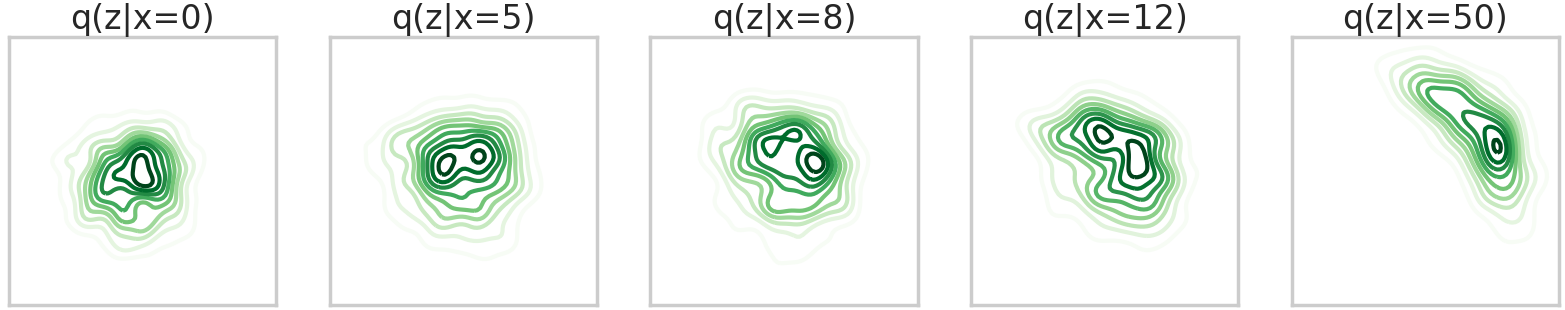
\includegraphics[width=\textwidth]{13963.png}
\caption{Average KL Divergence of 1.3963}
\end{subfigure}
}
\end{figure}
\end{frame}
\begin{frame}{Inference Experiment - Activation Function}{KL Divergence Plots}
\begin{figure}
\begin{subfigure}{0.49\textwidth}
\includegraphics[width=\linewidth]{truklmins/PCKLvsPCKLEXP.png}
\caption{Prior-Contrastive}
\end{subfigure}
\begin{subfigure}{0.49\textwidth}
\includegraphics[width=\linewidth]{truklmins/JCKLvsJCKLEXP.png}
\caption{Joint-Contrastive}
\end{subfigure}
\end{figure}
\end{frame}
\begin{frame}{Inference Experiment - Activation Function}{Estimator Losses}
\begin{figure}
\begin{subfigure}{0.49\textwidth}
\includegraphics[width=\linewidth]{estimator_losses/PCKLvsPCKLEXP.png}
\caption{Prior-Contrastive}
\end{subfigure}
\begin{subfigure}{0.49\textwidth}
\includegraphics[width=\linewidth]{estimator_losses/JCKLvsJCKLEXP.png}
\caption{Joint-Contrastive}
\end{subfigure}
\end{figure}
\end{frame}
\begin{frame}{Inference Experiment - Activation Function}{NELBOs}
\begin{figure}
\begin{subfigure}{0.49\textwidth}
\includegraphics[width=\linewidth]{nelbos/PCKLvsPCKLEXP.png}
\caption{Prior-Contrastive}
\end{subfigure}
\begin{subfigure}{0.49\textwidth}
\includegraphics[width=\linewidth]{nelbos/JCKLvsJCKLEXP.png}
\caption{Joint-Contrastive}
\end{subfigure}
\end{figure}
\end{frame}

\section{Theory Break}
\begin{frame}{Theory Break}{Alternative Derivation of Class Probability Estimation}
\begin{itemize}
\item Recall theorem behind divergence minimisation:
\[D_f [p(u)||q(u)]\geq \sup_{r\in \mathcal{R}} \{\mathbb{E}_{q(u)}[f'(r(u))]-\mathbb{E}_{p(u)}[f^*(f'(r(u)))]\},\]
\item If we let $f(u)=u\log u-(u+1)\log (u+1)$ and $D(u)=\frac{r(u)}{r(u)+1}$, we have the lower bound
\[2JS[p(u)||q(u)]-\log 4\geq \sup_{D}\{\E_{q(u)}[\log D(u)]+\E_{p(u)}[\log(1-D(u))]\}\]
\item This is the same estimator loss as in class probability estimation:
\[\min_\alpha -\mathbb{E}_{q(u)}[\log D_\alpha(u)]-\mathbb{E}_{p(u)}[\log(1-D_\alpha(u))]\]
\item We call $2JS[p(u)||q(u)]-\log 4$ the `GAN' divergence
\end{itemize}
\end{frame}
\begin{frame}{Theory Break}{Analysis of Optimisation Algorithms}
\begin{itemize}
\item $D(u)=\frac{r(u)}{r(u)+1}$ is bijective transformation of estimated density ratio.
\item Also propose  $T(u)=\log r(u)$.
\item 2 f-divergences being compared: $KL[q(u)||p(u)]$ and $2JS[p(u)||q(u)]-\log 4$.
\item 2 problem contexts (PC, JC) \\
$\times$ 2 f-divergences (Reverse KL, GAN) \\
$\times$ 3 estimator parametrisations ($D_\alpha(u)\simeq\frac{q(u)}{q(u)+p(u)}, r_\alpha(u)
\simeq\frac{q(u)}{p(u)}, T_\alpha(u)\simeq\log \frac{q(u)}{p(u)}$)\\
 = 12 experiments.
\end{itemize}
\end{frame}
\section{Experiments}
\subsection{Inference Experiment}
\begin{frame}{Inference Experiment}{Comparing Optimal Estimators}
\begin{itemize}
\item Same inference problem as before.
\item Aim of this experiment is to verify that choice of estimator does not matter as long as it reaches equality.
\item Low training rate with high estimator to posterior optimisation ratio (100:1).
\item High posterior iterations.
\end{itemize}
\end{frame}
\begin{frame}{Inference Experiment}{Comparing Optimal Estimators}
\begin{table}[h]
\scalebox{0.8}{
\begin{tabular}{|c|c|c|}
\hline
Algorithm & Mean KL Divergence & Standard Deviation\\
\hline
PC Reverse KL - $D_\alpha(z,x)$ & 1.3271 & 0.0041\\
\hline
PC Reverse KL - $r_\alpha(z,x)$ & 1.3265 & 0.0045\\
\hline
PC Reverse KL - $T_\alpha(z,x)$ & 1.3262 & 0.0041\\
\hline
PC CPE - $D_\alpha(z,x)$ & 1.3267 & 0.0041\\
\hline
PC GAN - $r_\alpha(z,x)$ & 1.3263 & 0.0035\\
\hline
PC GAN - $T_\alpha(z,x)$ & 1.3258 & 0.0039\\
\hline
JC Reverse KL - $D_\alpha(z,x)$ & 1.3416 & 0.0068\\
\hline
JC Reverse KL - $r_\alpha(z,x)$ & 1.3397 & 0.0066\\
\hline
JC Reverse KL - $T_\alpha(z,x)$ & 1.3446 & 0.0108\\
\hline
JC GAN - $D_\alpha(z,x)$ & 1.3648 & 0.0242\\
\hline
JC GAN - $r_\alpha(z,x)$ & 1.3657 & 0.0302\\
\hline
JC GAN - $T_\alpha(z,x)$ & 1.3670 & 0.0387\\
\hline
\end{tabular}
}
\end{table}
\begin{itemize}
\item PC posteriors fully converged, reverse KL converged faster for JC.
\end{itemize}
\end{frame}
\begin{frame}{Inference Experiment}{Prior-Contrastive KL Divergence Plots}
\begin{figure}
\begin{subfigure}{0.49\textwidth}
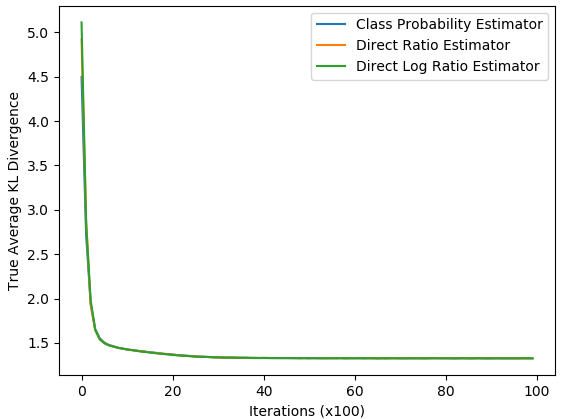
\includegraphics[width=\linewidth]{truklmins/PCADVvsPCADVexpvsPCADVgudlog.png}
\caption{GAN Divergence}
\end{subfigure}
\begin{subfigure}{0.49\textwidth}
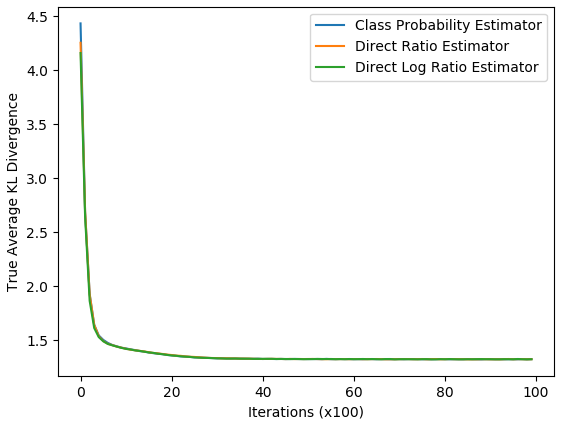
\includegraphics[width=\linewidth]{truklmins/PCKLDvsPCKLexpvsPCKLgudlog.png}
\caption{Reverse KL Divergence}
\end{subfigure}
\end{figure}
\end{frame}
\begin{frame}{Inference Experiment}{Joint-Contrastive KL Divergence Plots}
\begin{figure}
\begin{subfigure}{0.49\textwidth}
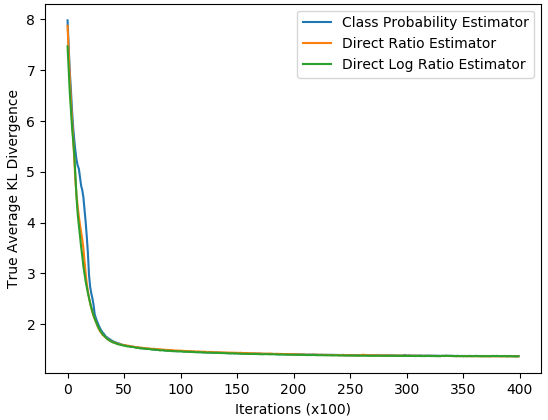
\includegraphics[width=\linewidth]{truklmins/JCADVvsJCADVexpvsJCADVgudlog.png}
\caption{GAN Divergence}
\end{subfigure}
\begin{subfigure}{0.49\textwidth}
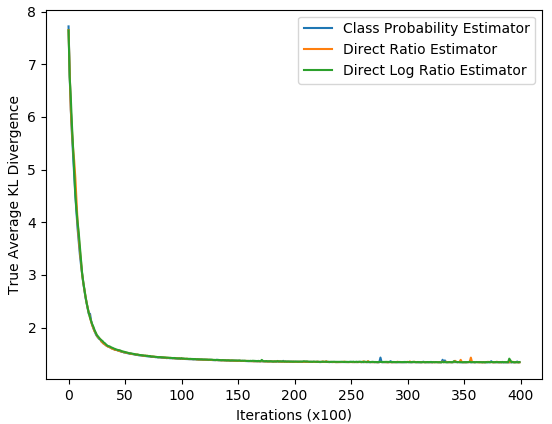
\includegraphics[width=\linewidth]{truklmins/JCKLDvsJCKLexpvsJCKLgudlog.png}
\caption{Reverse KL Divergence}
\end{subfigure}
\end{figure}
\end{frame}
\begin{frame}{Inference Experiment}{Prior-Contrastive Estimator Loss Plots}
\begin{figure}
\begin{subfigure}{0.49\textwidth}
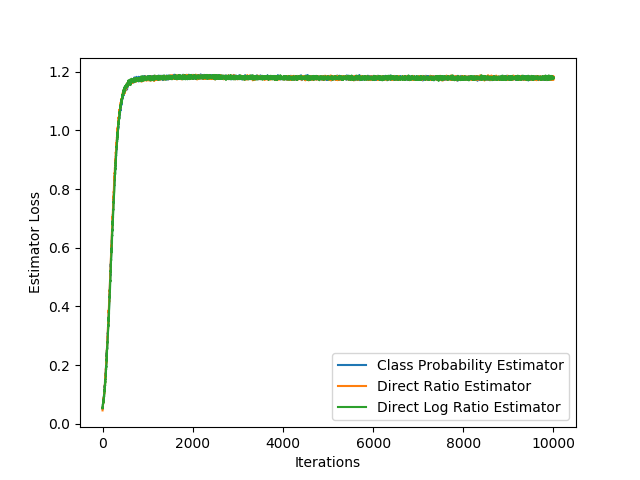
\includegraphics[width=\linewidth]{estimator_losses/PCADVvsPCADVexpvsPCADVgudlog.png}
\caption{GAN Divergence}
\end{subfigure}
\begin{subfigure}{0.49\textwidth}
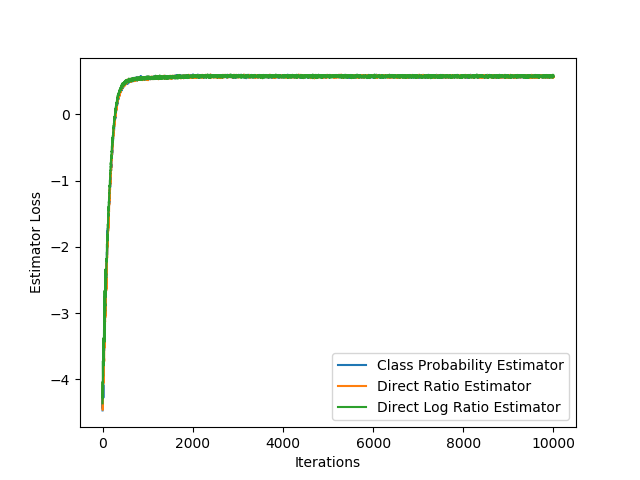
\includegraphics[width=\linewidth]{estimator_losses/PCKLDvsPCKLexpvsPCKLgudlog.png}
\caption{Reverse KL Divergence}
\end{subfigure}
\end{figure}
\end{frame}
\begin{frame}{Inference Experiment}{Joint-Contrastive Estimator Loss Plots}
\begin{figure}
\begin{subfigure}{0.49\textwidth}
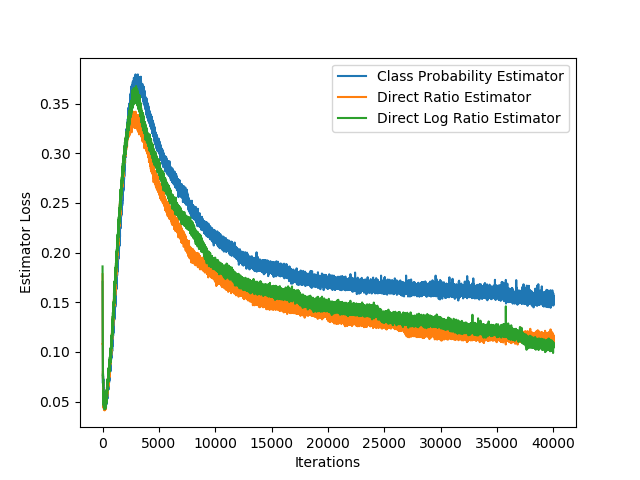
\includegraphics[width=\linewidth]{estimator_losses/JCADVvsJCADVexpvsJCADVgudlog.png}
\caption{GAN Divergence}
\end{subfigure}
\begin{subfigure}{0.49\textwidth}
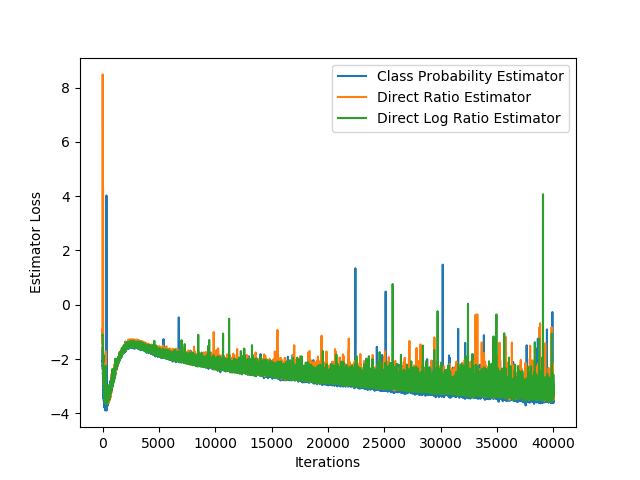
\includegraphics[width=\linewidth]{estimator_losses/JCKLDvsJCKLexpvsJCKLgudlog.png}
\caption{Reverse KL Divergence}
\end{subfigure}
\end{figure}
\end{frame}
\begin{frame}{Inference Experiment}{Prior-Contrastive NELBO Plots}
\begin{figure}
\begin{subfigure}{0.49\textwidth}
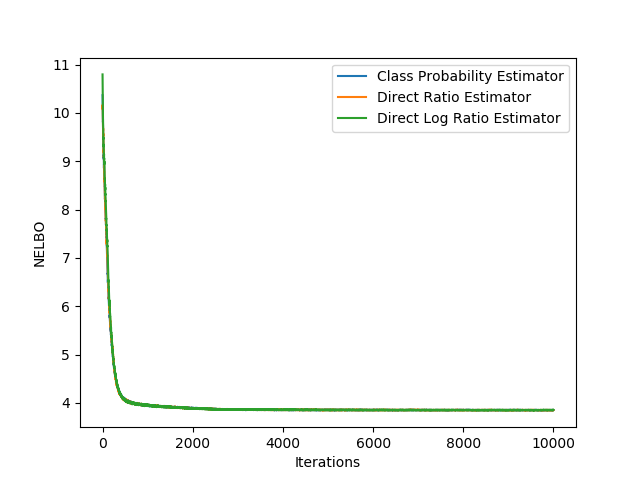
\includegraphics[width=\linewidth]{nelbos/PCADVvsPCADVexpvsPCADVgudlog.png}
\caption{GAN Divergence}
\end{subfigure}
\begin{subfigure}{0.49\textwidth}
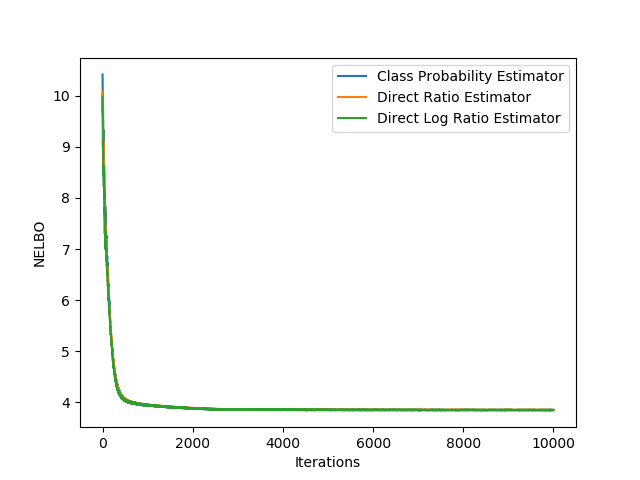
\includegraphics[width=\linewidth]{nelbos/PCKLDvsPCKLexpvsPCKLgudlog.png}
\caption{Reverse KL Divergence}
\end{subfigure}
\end{figure}
\end{frame}
\begin{frame}{Inference Experiment}{Joint-Contrastive NELBO Plots}
\begin{figure}
\begin{subfigure}{0.49\textwidth}
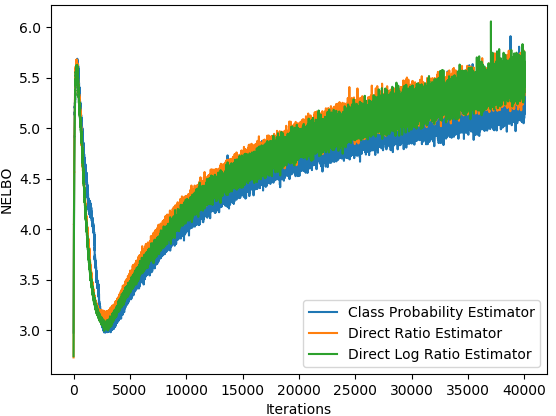
\includegraphics[width=\linewidth]{nelbos/JCADVvsJCADVexpvsJCADVgudlog.png}
\caption{GAN Divergence}
\end{subfigure}
\begin{subfigure}{0.49\textwidth}
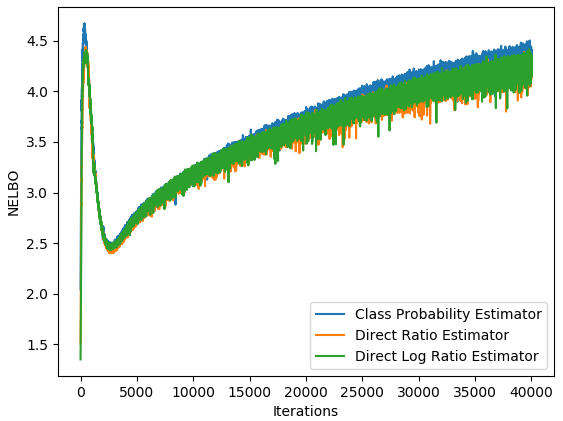
\includegraphics[width=\linewidth]{nelbos/JCKLDvsJCKLexpvsJCKLgudlog.png}
\caption{Reverse KL Divergence}
\end{subfigure}
\end{figure}
\end{frame}
\begin{frame}{Inference Experiment}{Comparing Undertrained Estimators}
\begin{itemize}
\item Aim of this experiment is to significantly reduce the amount of training the estimator undergoes between each NELBO estimation.
\item The combination of f-divergence and estimator parametrisation that trains the fastest will have the highest accuracy, corresponding to the highest posterior convergence.
\item Estimator training rate changed to 0.00004 and posterior training rate increased to 0.0002.
\item 5000 estimator initialisation steps retained.
\item Estimator to posterior iteration ratio reduced to 15:1 in prior-contrastive and 20:1 in joint-contrastive.
\item Total posterior iterations reduced to 2000 in prior-contrastive and 4000 in joint-contrastive.
\end{itemize}
\end{frame}
\begin{frame}{Inference Experiment}{Comparing Undertrained Estimators}
\begin{table}[h]
\scalebox{0.8}{
\begin{tabular}{|c|c|c|}
\hline
Algorithm & Mean KL Divergence & Standard Deviation\\
\hline
PC Reverse KL - $D_\alpha(z,x)$ & 1.3572 & 0.0136\\
\hline
PC Reverse KL - $r_\alpha(z,x)$ & 1.3607 & 0.0199\\
\hline
PC Reverse KL - $T_\alpha(z,x)$ & 1.3641 & 0.0141\\
\hline
PC GAN - $D_\alpha(z,x)$ & 1.3788 & 0.0258\\
\hline
PC GAN - $r_\alpha(z,x)$ & 1.3811 & 0.0365\\
\hline
PC GAN - $T_\alpha(z,x)$ & 1.3849 & 0.0450\\
\hline
JC Reverse KL - $D_\alpha(z,x)$ & 1.3786 & 0.0286\\
\hline
JC Reverse KL - $r_\alpha(z,x)$ & 1.3934 & 0.0410\\
\hline
JC Reverse KL - $T_\alpha(z,x)$ & 1.4133 & 0.0597\\
\hline
JC GAN - $D_\alpha(z,x)$ & 1.4017 & 0.0286\\
\hline
JC GAN - $r_\alpha(z,x)$ & 1.4086 & 0.0555\\
\hline
JC GAN - $T_\alpha(z,x)$ & 1.4214 & 0.0518\\
\hline
\end{tabular}
}
\end{table}
\begin{itemize}
\item Reverse KL divergence significantly better than GAN divergence.

\end{itemize}
\end{frame}
\begin{frame}{Inference Experiment}{Comparing Undertrained Estimators}
\begin{itemize}
\item For PC, $D_\alpha(z,x)<r_\alpha(z,x)<T_\alpha(z,x)$ in terms of mean KL divergence but not by a significant amount.
\item Significant in JC. Likely because likelihood term is a factor in PC but JC is entirely based on density ratio.
\item Standard deviation of class probability estimator consistently better than other two estimator parametrisations.
\item f-divergence used is more significant than estimator parametrisation.
\item Optimal combination is reverse KL divergence with class probability estimator.
\end{itemize}
\end{frame}
\begin{frame}{Inference Experiment}{Prior-Contrastive KL Divergence Plots}
\begin{figure}
\begin{subfigure}{0.49\textwidth}
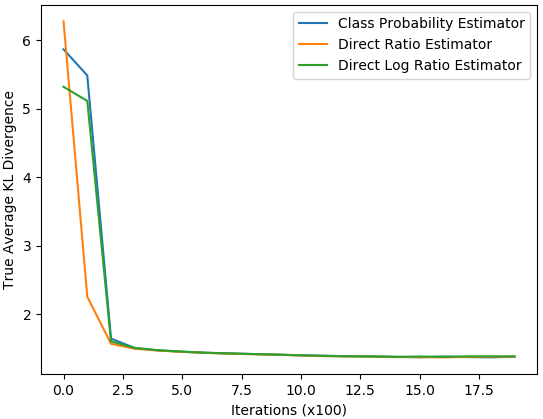
\includegraphics[width=\linewidth]{part2truklmins/PCADVvsPCADVexpvsPCADVgudlog.png}
\caption{GAN Divergence}
\end{subfigure}
\begin{subfigure}{0.49\textwidth}
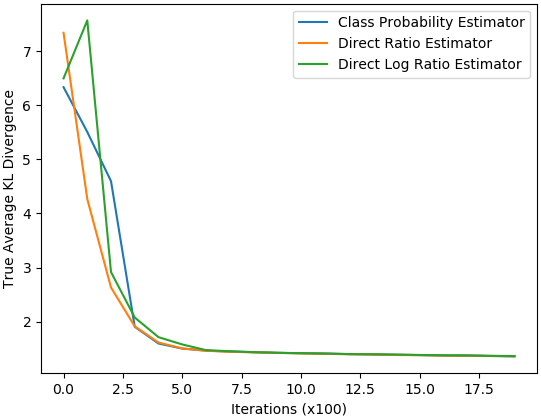
\includegraphics[width=\linewidth]{part2truklmins/PCKLDvsPCKLexpvsPCKLgudlog.png}
\caption{Reverse KL Divergence}
\end{subfigure}
\end{figure}
\end{frame}
\begin{frame}{Inference Experiment}{Joint-Contrastive KL Divergence Plots}
\begin{figure}
\begin{subfigure}{0.49\textwidth}
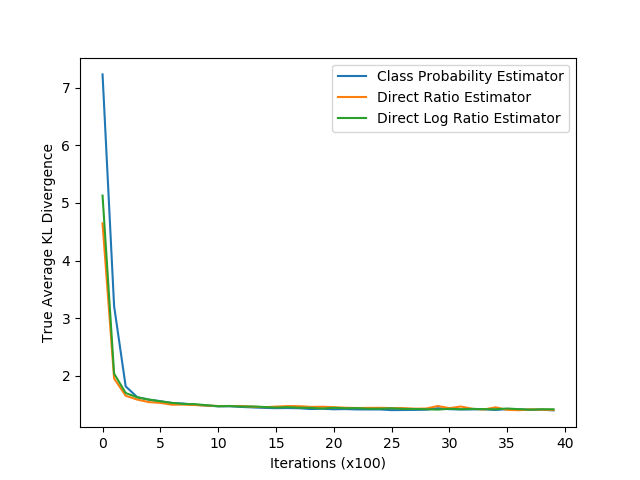
\includegraphics[width=\linewidth]{part2truklmins/JCADVvsJCADVexpvsJCADVgudlog.png}
\caption{GAN Divergence}
\end{subfigure}
\begin{subfigure}{0.49\textwidth}
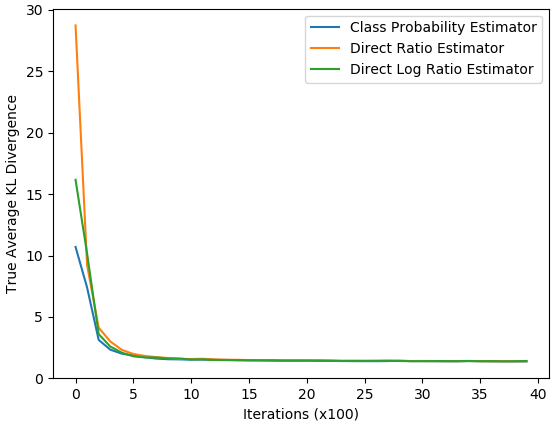
\includegraphics[width=\linewidth]{part2truklmins/JCKLDvsJCKLexpvsJCKLgudlog.png}
\caption{Reverse KL Divergence}
\end{subfigure}
\end{figure}
\end{frame}
\begin{frame}{Inference Experiment}{Prior-Contrastive Estimator Loss Plots}
\begin{figure}
\begin{subfigure}{0.49\textwidth}
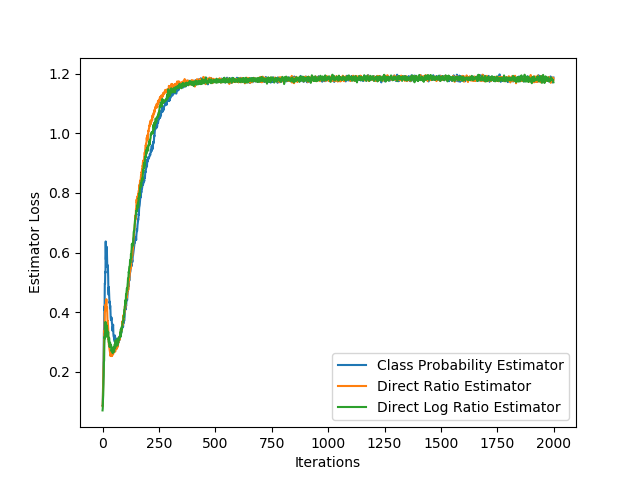
\includegraphics[width=\linewidth]{part2estimatorlosses/PCADVvsPCADVexpvsPCADVgudlog.png}
\caption{GAN Divergence}
\end{subfigure}
\begin{subfigure}{0.49\textwidth}
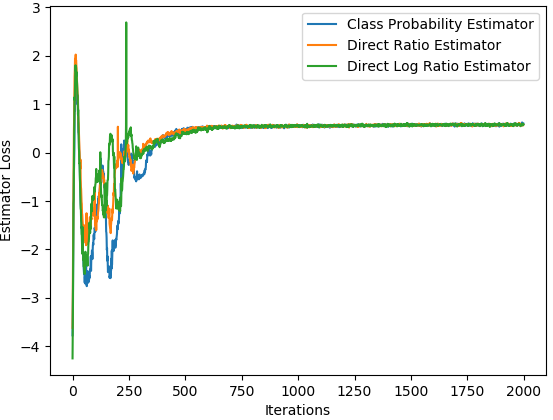
\includegraphics[width=\linewidth]{part2estimatorlosses/PCKLDvsPCKLexpvsPCKLgudlog.png}
\caption{Reverse KL Divergence}
\end{subfigure}
\end{figure}
\end{frame}
\begin{frame}{Inference Experiment}{Joint-Contrastive Estimator Loss Plots}
\begin{figure}
\begin{subfigure}{0.49\textwidth}
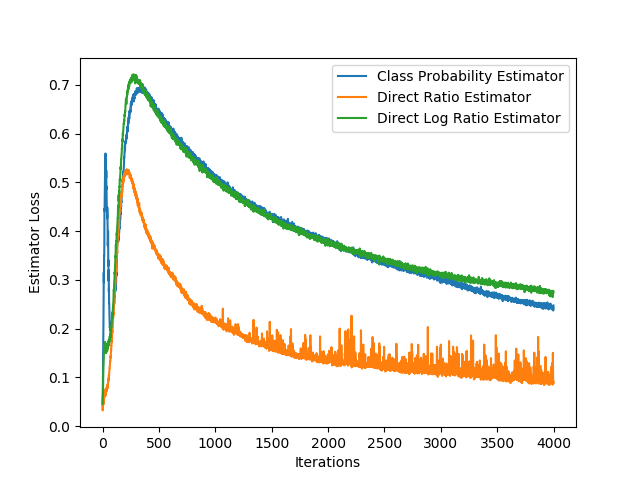
\includegraphics[width=\linewidth]{part2estimatorlosses/JCADVvsJCADVexpvsJCADVgudlog.png}
\caption{GAN Divergence}
\end{subfigure}
\begin{subfigure}{0.49\textwidth}
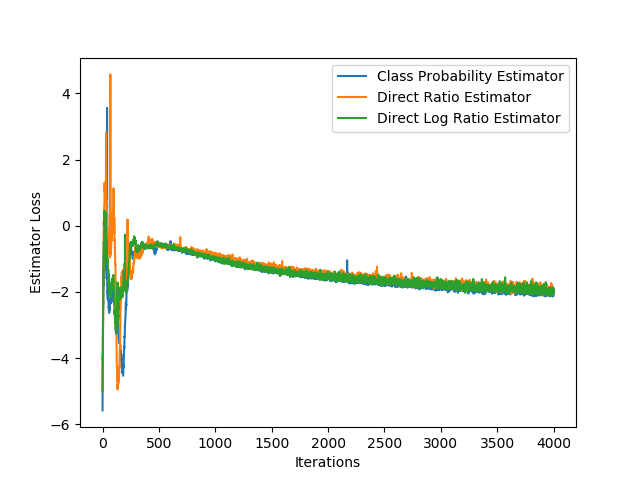
\includegraphics[width=\linewidth]{part2estimatorlosses/JCKLDvsJCKLexpvsJCKLgudlog.png}
\caption{Reverse KL Divergence}
\end{subfigure}
\end{figure}
\end{frame}
\begin{frame}{Inference Experiment}{Prior-Contrastive NELBO Plots}
\begin{figure}
\begin{subfigure}{0.49\textwidth}
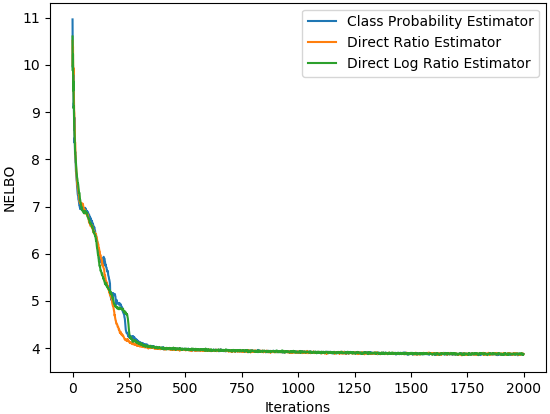
\includegraphics[width=\linewidth]{part2nelbos/PCADVvsPCADVexpvsPCADVgudlog.png}
\caption{GAN Divergence}
\end{subfigure}
\begin{subfigure}{0.49\textwidth}
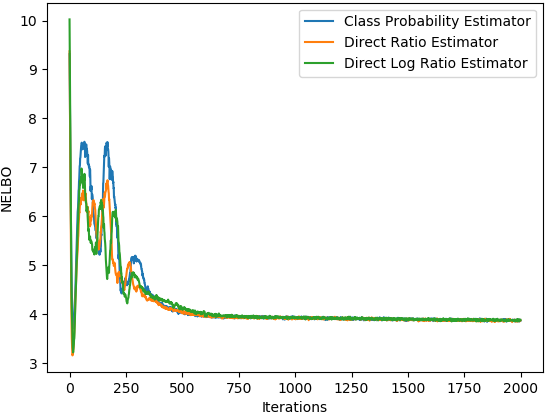
\includegraphics[width=\linewidth]{part2nelbos/PCKLDvsPCKLexpvsPCKLgudlog.png}
\caption{Reverse KL Divergence}
\end{subfigure}
\end{figure}
\end{frame}
\begin{frame}{Inference Experiment}{Joint-Contrastive NELBO Plots}
\begin{figure}
\begin{subfigure}{0.49\textwidth}
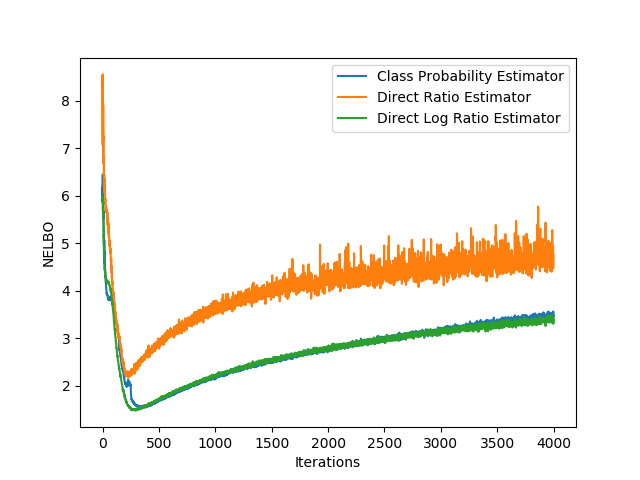
\includegraphics[width=\linewidth]{part2nelbos/JCADVvsJCADVexpvsJCADVgudlog.png}
\caption{GAN Divergence}
\end{subfigure}
\begin{subfigure}{0.49\textwidth}
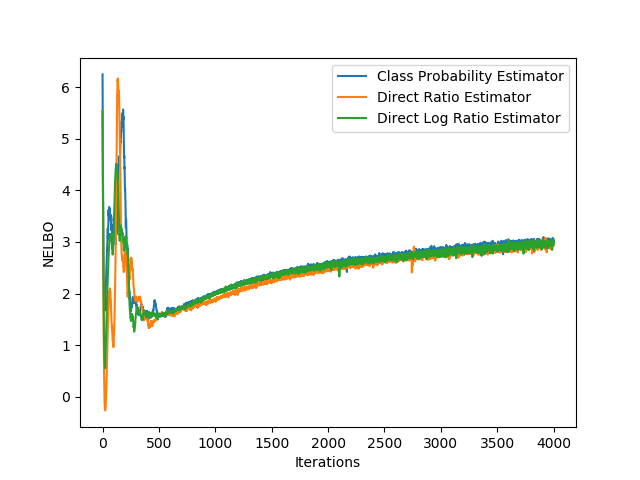
\includegraphics[width=\linewidth]{part2nelbos/JCKLDvsJCKLexpvsJCKLgudlog.png}
\caption{Reverse KL Divergence}
\end{subfigure}
\end{figure}
\end{frame}
\subsection{Generation Experiment}
\begin{frame}{Generation Experiment}{Autoencoders}
\begin{itemize}
\item Likelihood $p_\theta(x|z)$ is now a neural network.
\item Posterior $q_\phi(z|x)$ represents data $x$ as lower dimensional latent $z$.
\item Likelihood $p_\theta(x|z)$ reconstructs data $\tilde{x}$ from $z$.
\item Generate new data $\tilde{x}$ using $z$ from $p(z)$.
\end{itemize}
\begin{figure}[h]
  \centering
  \scalebox{0.8}{
  \tikz{ %
    \node[latent] (x) {$\bm{x}$} ; %
    \node[det, right=of x] (q) {$q_\phi(z|x)$} ; %
    \node [latent, above=of x] (eps) {$\epsilon$} ;
    \node [latent, right=of q] (z) {$\bm{z}$} ;
    \node [det, right=of z] (p) {$p_\theta(x|z)$} ;
    \node [latent, right=of p] (pout) {$\tilde{\bm{x}}$} ;
    \edge {x} {q} ; %
    \edge {q} {z} ;
    \edge {eps} {q} ;
    \edge {z} {p} ;
    \edge {p} {pout} ;
  }
  }
\end{figure}
\[\min_{\theta, \phi} -\mathbb{E}_{q_\phi(z|x)q^*(x)}[\log p_\theta(x|z)]+\mathbb{E}_{q^*(x)}[KL(q_\phi(z|x)||p(z))]\]
\end{frame}
\begin{frame}{Generation Experiment}{Experiment Outline}
\begin{itemize}
\item MNIST dataset - $28\times 28$ grey-scale images of handwritten digits
\item Not doing joint-contrastive cause unintuitive to `pretend' we don't know likelihood function.
\item Again use low estimator to posterior training ratio.
\item Use reconstruction error $\|x-\tilde{x}\|^2$ as metric.
\item Perform experiment with low dimensional latent space (2 dimensions) and high dimensional latent space (20 dimensions).
\end{itemize}
\end{frame}
\begin{frame}{Generation Experiment}{Results - low dimensional latent space}
\begin{table}[h]
\scalebox{0.9}{
\begin{tabular}{|c|c|c|}
\hline
Algorithm & Mean Reconstruction Error & Standard Deviation\\
\hline
PC Reverse KL - $D_\alpha(z,x)$ & 0.0866 & 0.0015\\
\hline
PC Reverse KL - $r_\alpha(z,x)$ & 0.0871 & 0.0021\\
\hline
PC Reverse KL - $T_\alpha(z,x)$ & 0.0873 & 0.0016\\
\hline
PC GAN - $D_\alpha(z,x)$ & 0.0867 & 0.0013\\
\hline
PC GAN - $r_\alpha(z,x)$ & 0.0872 & 0.0015\\
\hline
PC GAN - $T_\alpha(z,x)$ & 0.1068 & 0.0020\\
\hline
\end{tabular}
}
\end{table}
\begin{itemize}
\item Mostly insignificant but consistent results.
\item Log ratio estimator for GAN is significantly worse.
\end{itemize}
\end{frame}
\begin{frame}{Generation Experiment}{Reconstruction Errors}
\begin{figure}
\begin{subfigure}{0.49\textwidth}
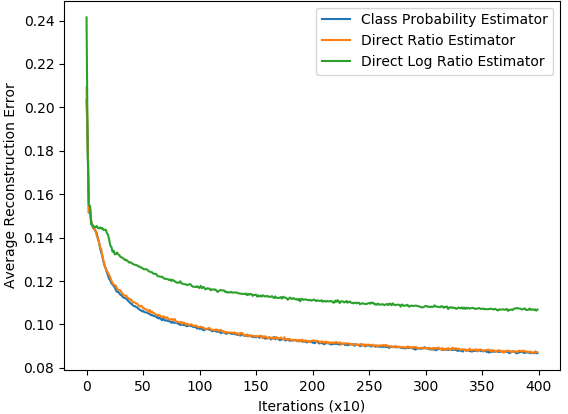
\includegraphics[width=\linewidth]{part3reconerrors/PCADVvsPCADVexpvsPCADVgudlog.png}
\caption{GAN Divergence}
\end{subfigure}
\begin{subfigure}{0.49\textwidth}
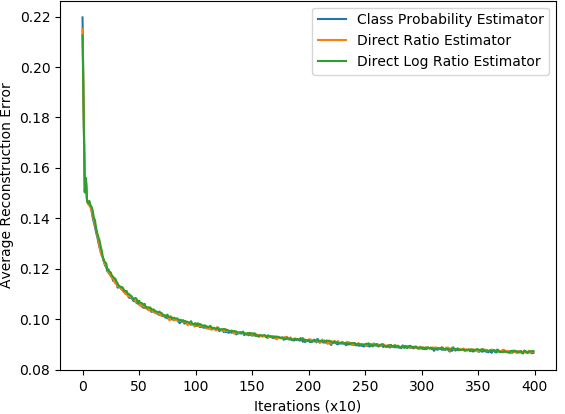
\includegraphics[width=\linewidth]{part3reconerrors/PCKLDvsPCKLexpvsPCKLgudlog.png}
\caption{Reverse KL Divergence}
\end{subfigure}
\end{figure}
\end{frame}
\begin{frame}{Generation Experiment}{Results - high dimensional latent space}
\begin{itemize}
\item Direct ratio and direct log ratio estimators attempted to store numbers exceeding float64(max).
\item Exponential of $T_\alpha(z,x)$ taken in loss function.
\item $D_\alpha(z,x)$ ranges in $(0,1)$.
\item Value before sigmoid activation function for $D_\alpha(z,x)$ is log density ratio.
\item Class probability estimator is the best.
\end{itemize}
\end{frame}
\begin{frame}{Generation Experiment}{Results - high dimensional latent space}
\begin{figure}
\begin{subfigure}{0.49\textwidth}
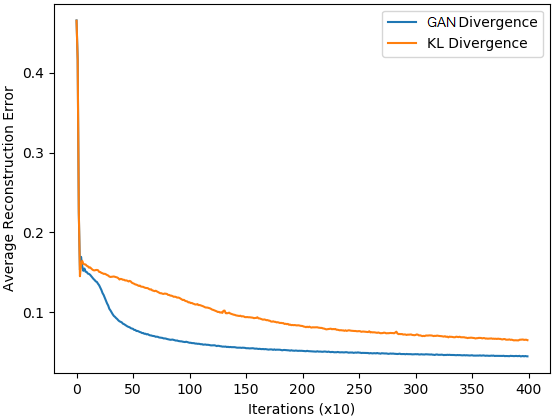
\includegraphics[width=\linewidth]{part4reconerrors/PCADVvsPCKLD.png}
\caption{Reconstruction Error}
\end{subfigure}
\begin{subfigure}{0.49\textwidth}
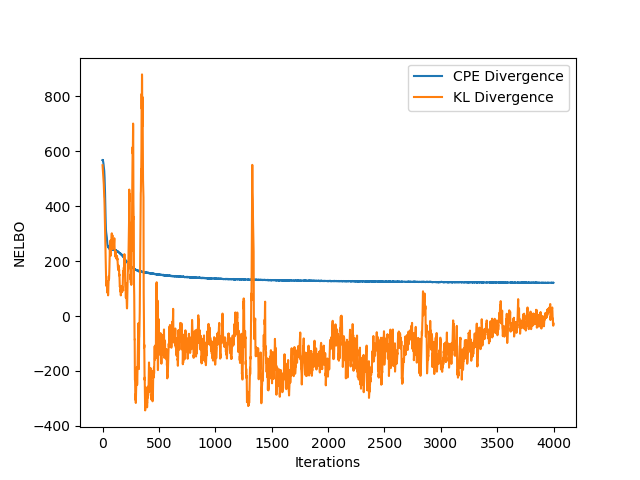
\includegraphics[width=\linewidth]{part4nelbos/PCADVvsPCKLD.png}
\caption{NELBO}
\end{subfigure}
\end{figure}
\begin{table}[h]
\scalebox{0.9}{
\begin{tabular}{|c|c|c|}
\hline
Algorithm & Mean Reconstruction Error & Standard Deviation\\
\hline
PC Reverse KL - $D_\alpha(z,x)$ & 0.0444 & 0.0017\\
\hline
PC GAN - $D_\alpha(z,x)$ & 0.0647 & 0.0019\\
\hline
\end{tabular}
}
\end{table}
\end{frame}
%\begin{frame}{Blocks}
%\begin{block}{Block Title}
%You can also highlight sections of your presentation in a block, with it's own title
%\end{block}
%\begin{theorem}
%There are separate environments for theorems, examples, definitions and proofs.
%\end{theorem}
%\begin{example}
%Here is an example of an example block.
%\end{example}
%\end{frame}

% Placing a * after \section means it will not show in the
% outline or table of contents.
\section{Further Estimator Loss Function Analysis}
\begin{frame}{Further Estimator Loss Function Analysis}{Outline}
\begin{itemize}
\item Each estimator loss function is a convex functional that reaches its minimum when estimator is optimal.
\item Estimator parametrisation affects its output space and gradient of loss function with respect to the estimator.
\item Choice of f-divergence affects gradient of loss function with respect to estimator.
\end{itemize}
\end{frame}
\begin{frame}{Further Estimator Loss Function Analysis}{Estimator Parametrisation}
Need some plots xD
\begin{itemize}
\item Higher second derivative corresponds to faster convergence.
\item Taking second functional derivative of estimator loss function with respect to estimator, we can only make one certain comparison: for the GAN divergence, the class probability estimator has a strictly higher second derivative than the direct ratio estimator.
\item The density ratio changes every time the posterior is optimised, and the estimator must catch up. It can be shown that the class probability estimator has a strictly lower displacement than the direct ratio estimator, that is, $|D^*_{final}-D^*_{init}|<|r^*_{final}-r^*_{init}|$.
\end{itemize}
\end{frame}
\begin{frame}{Further Estimator Loss Function Analysis}{Choice of f-divergence}
\begin{itemize}
\item Again observing the second functional derivatives, we can only observe that in the direct ratio estimator parametrisation, the reverse KL divergence is strictly higher than the GAN divergence.
\item Nowozin's f-GAN paper also shows empirically that the reverse KL divergence is superior when it is additionally used to optimize the posterior.
\end{itemize}
\end{frame}

\section*{Summary}

\begin{frame}{Summary}
  \begin{itemize}
  \item
    The \alert{first main message} of your talk in one or two lines.
  \item
    The \alert{second main message} of your talk in one or two lines.
  \item
    Perhaps a \alert{third message}, but not more than that.
  \end{itemize}
  
  \begin{itemize}
  \item
    Outlook
    \begin{itemize}
    \item
      Something you haven't solved.
    \item
      Something else you haven't solved.
    \end{itemize}
  \end{itemize}
\end{frame}



% All of the following is optional and typically not needed. 
\appendix
\section<presentation>*{\appendixname}
\subsection<presentation>*{For Further Reading}

\begin{frame}[allowframebreaks]
  \frametitle<presentation>{For Further Reading}
    
  \begin{thebibliography}{10}
    
  \beamertemplatebookbibitems
  % Start with overview books.

  \bibitem{Author1990}
    A.~Author.
    \newblock {\em Handbook of Everything}.
    \newblock Some Press, 1990.
 
    
  \beamertemplatearticlebibitems
  % Followed by interesting articles. Keep the list short. 

  \bibitem{Someone2000}
    S.~Someone.
    \newblock On this and that.
    \newblock {\em Journal of This and That}, 2(1):50--100,
    2000.
  \end{thebibliography}
\end{frame}

\end{document}


